\documentclass[12pt,a4paper]{article}
\usepackage[utf8]{inputenc}
\usepackage[T1]{fontenc}
\usepackage{amsmath, amssymb, amsfonts}
\usepackage{graphicx}
\usepackage{float}
\usepackage{geometry}
\usepackage{xcolor}
\geometry{margin=2.5cm}

\title{Diferenčne metode za parcialne diferencialne enačbe}
\author{Filip Jesenšek (28231064)}
\date{\today}

\begin{document}

\maketitle

\begin{abstract}
V poročilu obravnavamo numerično reševanje časovne Schrödingerjeve enačbe v eni dimenziji z uporabo Crank-Nicolsonove metode. Primerjamo različne rede natančnosti prostorske diskretizacije drugega odvoda ter različne pristope k časovnemu korakanju. V prvem delu analiziramo koherentno stanje v harmoničnem potencialu, kjer preverjamo ohranjanje verjetnosti in natančnost numerične rešitve. V drugem delu obravnavamo Gaussov valovni paket v prostem prostoru, kjer opazujemo grupno in fazno hitrost. Na koncu primerjamo vpliv višjih redov diferenčnih shem na natančnost rešitve.
\end{abstract}

\section{Uvod}

Enorazsežna nestacionarna Schrödingerjeva enačba je osnovno orodje za nerelativistični opis časovnega razvoja kvantnih stanj v različnih potencialih. Zapišemo jo kot:

\begin{equation}
\left( i\hbar \frac{\partial}{\partial t} - H \right) \psi(x, t) = 0,
\end{equation}

kjer je Hamiltonov operator v naravnih enotah ($\hbar = m = 1$) podan z:

\begin{equation}
H = -\frac{1}{2} \frac{\partial^2}{\partial x^2} + V(x).
\end{equation}

Razvoj stanja $\psi(x, t)$ v stanje $\psi(x, t + \Delta t)$ lahko opišemo s Padéjevim približkom eksponentne funkcije:

\begin{equation}
\psi(x, t + \Delta t) = e^{-iH\Delta t} \psi(x, t) \approx \frac{1 - \frac{1}{2}iH\Delta t}{1 + \frac{1}{2}iH\Delta t} \psi(x, t),
\end{equation}

ki je unitaren in reda $O(\Delta t^3)$. Ta približek je znan kot Crank-Nicolsonova metoda.

\subsection{Prostorska diskretizacija}

Območje $a \leq x \leq b$ diskretiziramo na krajevno mrežo $x_j = a + j\Delta x$ pri $0 \leq j < N$, kjer je $\Delta x = (b - a)/(N - 1)$. Drugi odvod v točki $x_j$ lahko aproksimiramo z diferenčnimi shemami različnih redov:

\begin{itemize}
    \item \textbf{2. red} (tritočkovna shema):
    \begin{equation}
    \psi''(x) \approx \frac{\psi_{j+1} - 2\psi_j + \psi_{j-1}}{\Delta x^2}
    \end{equation}
    
    \item \textbf{4. red} (pettočkovna shema):
    \begin{equation}
    \psi''(x) \approx \frac{-\psi_{j-2} + 16\psi_{j-1} - 30\psi_j + 16\psi_{j+1} - \psi_{j+2}}{12\Delta x^2}
    \end{equation}
    
    \item \textbf{6. red} (sedemtočkovna shema):
    \begin{equation}
    \psi''(x) \approx \frac{2\psi_{j-3} - 27\psi_{j-2} + 270\psi_{j-1} - 490\psi_j + 270\psi_{j+1} - 27\psi_{j+2} + 2\psi_{j+3}}{180\Delta x^2}
    \end{equation}
    
    \item \textbf{8. red} (devettočkovna shema):
    \begin{equation}
    \psi''(x) \approx \frac{-\frac{1}{560}\psi_{j-4} + \frac{8}{315}\psi_{j-3} - \frac{1}{5}\psi_{j-2} + \frac{8}{5}\psi_{j-1} - \frac{205}{72}\psi_j + \frac{8}{5}\psi_{j+1} - \frac{1}{5}\psi_{j+2} + \frac{8}{315}\psi_{j+3} - \frac{1}{560}\psi_{j+4}}{\Delta x^2}
    \end{equation}
\end{itemize}

\subsection{Matrična formulacija}

Ko diferenčne približke vstavimo v Crank-Nicolsonovo shemo, dobimo sistem linearnih enačb:

\begin{equation}
\mathbf{A} \Psi^{n+1} = \mathbf{A}^* \Psi^n,
\end{equation}

kjer sta matriki $\mathbf{A}$ in $\mathbf{A}^*$ definirani kot:

\begin{equation}
\mathbf{A} = \mathbf{I} + \frac{i\Delta t}{2}\mathbf{H}, \qquad \mathbf{A}^* = \mathbf{I} - \frac{i\Delta t}{2}\mathbf{H}.
\end{equation}

Hamiltonovo matriko $\mathbf{H}$ sestavimo iz kinetičnega člena (matrika drugega odvoda) in diagonalne matrike potenciala:

\begin{equation}
\mathbf{H} = -\frac{1}{2} \mathbf{D}_2 + \operatorname{diag}(V(x_j)).
\end{equation}

\section{Naloga}

Spremljaj časovni razvoj začetnega stanja:

\begin{equation}
\Psi(x, 0) = \sqrt{\frac{\alpha}{\sqrt{\pi}}} e^{-\alpha^2(x-\lambda)^2/2}
\end{equation}

v harmoničnem potencialu $V(x) = \frac{1}{2}kx^2$, kjer je v naravnih enotah $\alpha = k^{1/4}$, $\omega = \sqrt{k}$. Analitična rešitev je koherentno stanje:

\begin{equation}
\psi(x, t) = \sqrt{\frac{\alpha}{\sqrt{\pi}}} \exp\left[-\frac{1}{2}(\xi - \xi_{\lambda} \cos \omega t)^2 - i\left(\frac{\omega t}{2} + \xi \xi_{\lambda} \sin \omega t - \frac{1}{4} \xi_{\lambda}^2 \sin 2\omega t\right)\right],
\end{equation}

kjer je $\xi = \alpha x$, $\xi_{\lambda} = \alpha \lambda$. Parametri so: $\omega = 0,2$, $\lambda = 10$. Krajevno mrežo vpni v interval $[a, b] = [-40, 40]$ z $N = 300$ aktivnimi točkami. Nihajni čas je $T = 2\pi/\omega$. Stanje opazuj deset period.

Opazuj še razvoj Gaussovega valovnega paketa:

\begin{equation}
\psi(x, 0) = (2\pi\sigma_0^2)^{-1/4} e^{ik_0(x-\lambda)} e^{-(x-\lambda)^2/(2\sigma_0)^2}
\end{equation}

v prostoru brez potenciala. Parametri: $\sigma_0 = 1/20$, $k_0 = 50\pi$, $\lambda = 0,25$ in območje $[a, b] = [-0,5, 1,5]$ ter $\Delta t = 2\Delta x^2$. Časovni razvoj spremljaj, dokler težišče paketa ne pride do $x \approx 0,75$. Analitična rešitev je:

\begin{equation}
\psi(x, t) = \frac{(2\pi\sigma_0^2)^{-1/4}}{\sqrt{1 + \mathrm{i}t/(2\sigma_0^2)}} \exp\left[-\frac{(x-\lambda)^2/(2\sigma_0)^2 + \mathrm{i}k_0(x-\lambda) - \mathrm{i}k_0^2 t/2}{1 + \mathrm{i}t/(2\sigma_0^2)}\right]
\end{equation}

\section{Rezultati in analiza}

\subsection{Harmonični oscilator - koherentno stanje}

Slika \ref{fig:harmonic} prikazuje časovni razvoj valovne funkcije v harmoničnem potencialu. Na levem grafikonu (a) je prikazana absolutna vrednost valovne funkcije $|\psi(x,t)|^2$, ki predstavlja verjetnostno gostoto. Na desnem grafikonu (b) je prikazan realni del valovne funkcije $\operatorname{Re}(\psi(x,t))$, ki razkriva notranjo fazno strukturo koherentnega stanja.

\begin{figure}[H]
    \centering
    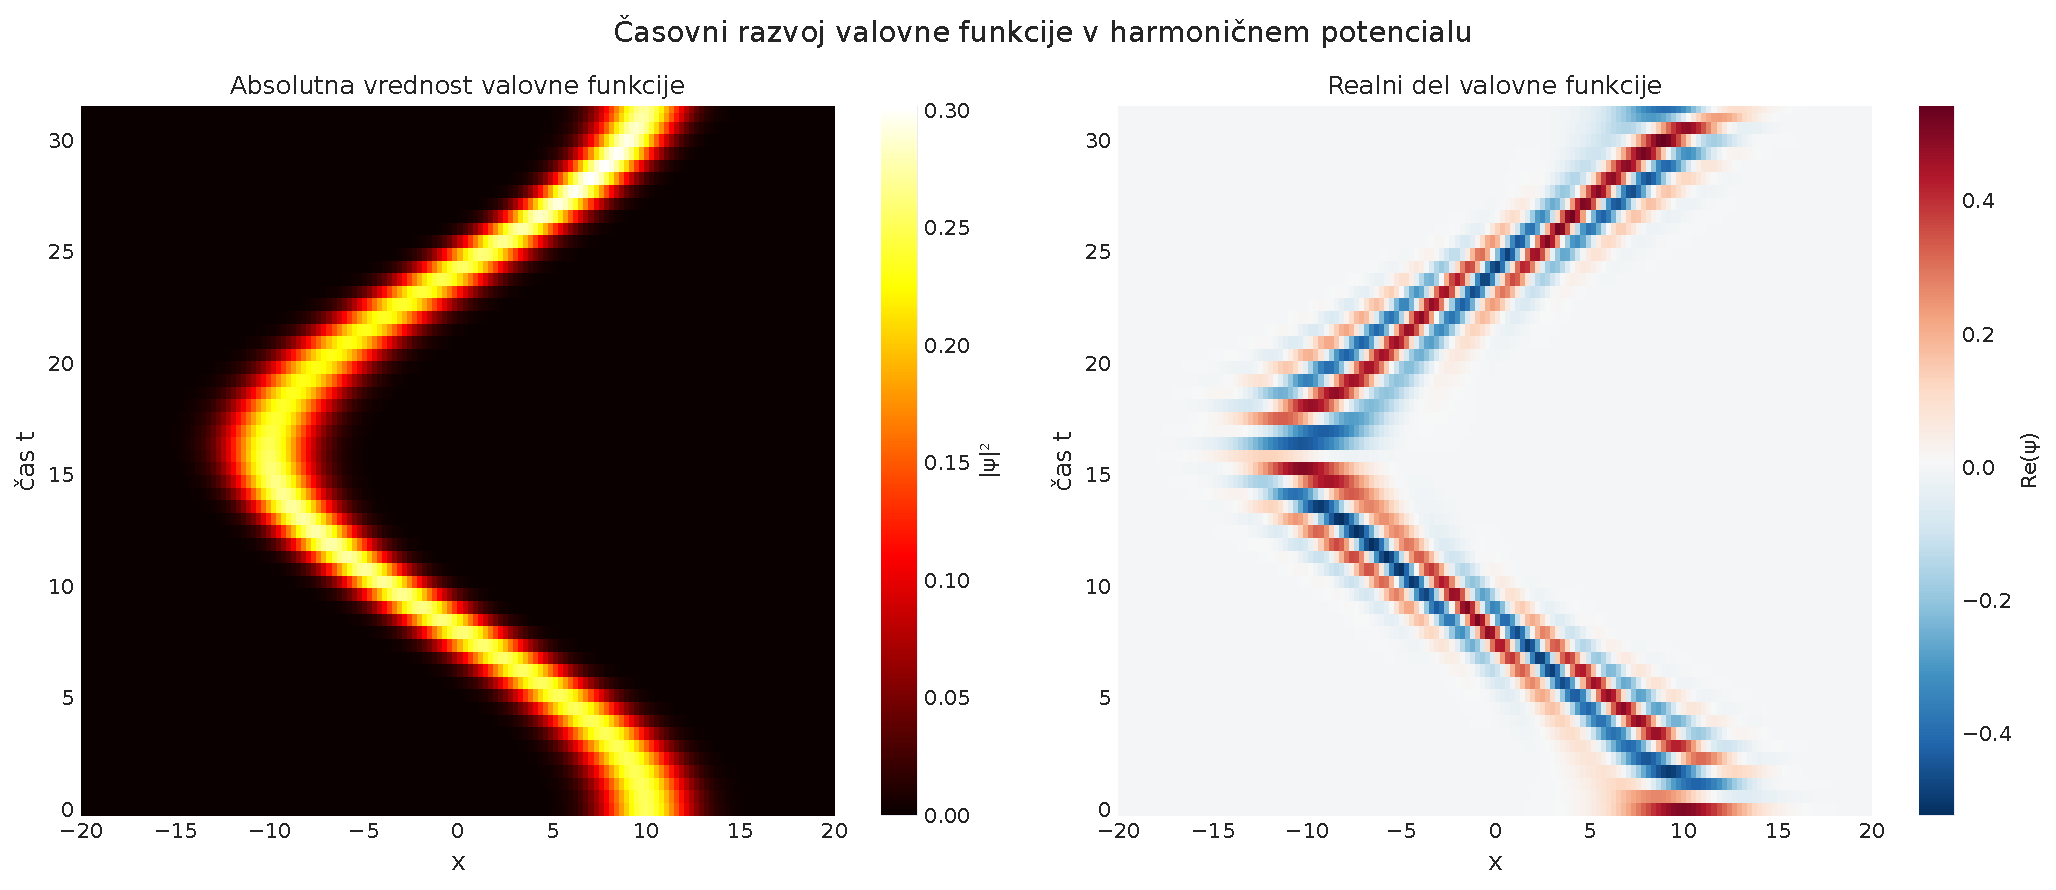
\includegraphics[width=0.9\textwidth]{harmonic_oscillator_heatmap.pdf}
    \caption{Časovni razvoj valovne funkcije v harmoničnem potencialu za $\omega = 0,2$, $\lambda = 10$. (a) Absolutna vrednost (verjetnostna gostota). (b) Realni del valovne funkcije.}
    \label{fig:harmonic}
\end{figure}

Iz slike je razvidno, da koherentno stanje ohranja svojo obliko med nihanjem, kar je značilnost harmoničnega oscilatorja. Težišče valovnega paketa niha sinusno okoli ravnovesne lege, kar je v skladu s korespondenčnim načelom – kvantno koherentno stanje se obnaša podobno kot klasičen oscilator. Na desnem grafikonu opazimo drobno strukturo realnega dela, ki izvira iz časovno odvisne faze valovne funkcije.

\subsection{Prosti delec - Gaussov valovni paket}

Slika \ref{fig:free} prikazuje časovni razvoj Gaussovega valovnega paketa v prostoru brez potenciala. Valovni paket se giblje v desno s grupno hitrostjo $v_g = k_0 = 50\pi$.

\begin{figure}[H]
    \centering
    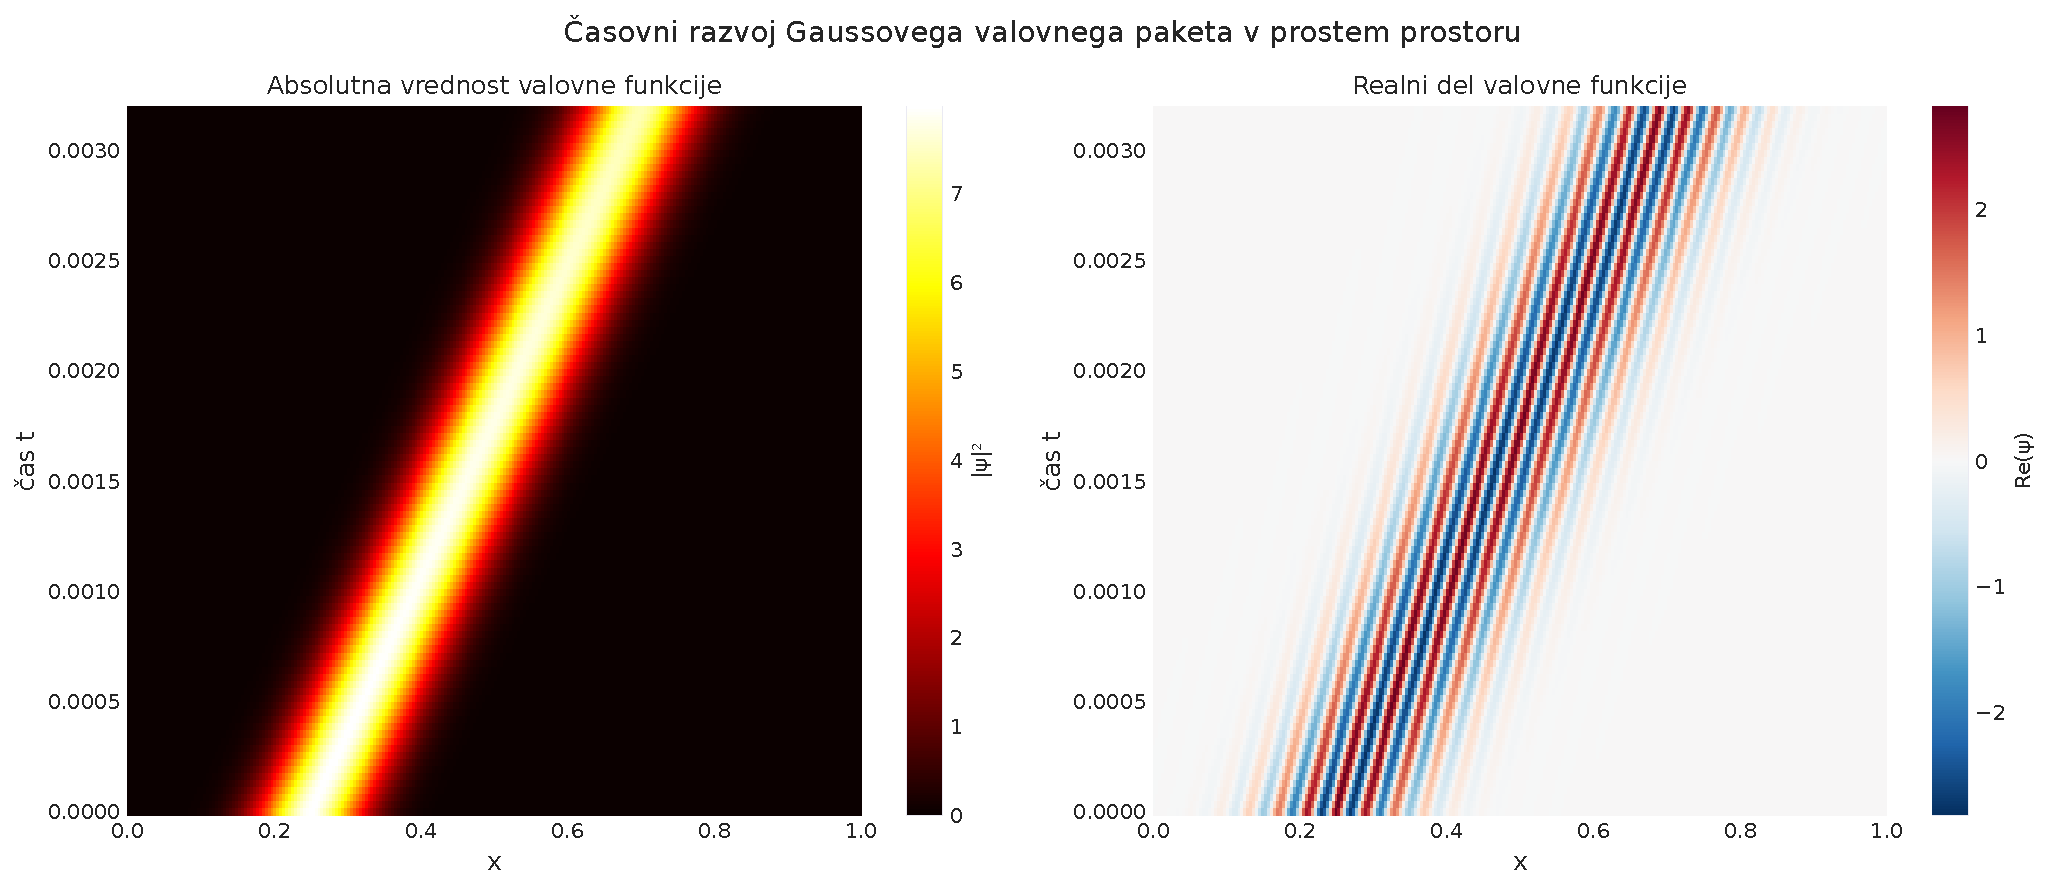
\includegraphics[width=0.9\textwidth]{free_particle_heatmap.pdf}
    \caption{Časovni razvoj Gaussovega valovnega paketa v prostem prostoru za $\sigma_0 = 1/20$, $k_0 = 50\pi$, $\lambda = 0,25$. (a) Absolutna vrednost (verjetnostna gostota). (b) Realni del valovne funkcije.}
    \label{fig:free}
\end{figure}

Na levem grafikonu opazimo, da se paket premika enakomerno v desno. Robovi paketa so nekoliko svetlejši, kar nakazuje na širjenje paketa, vendar je zaradi kratkega časa simulacije ta efekt še komaj opazen. Na desnem grafikonu vidimo izokrome (črte konstantne faze), ki so nagnjene pod manjšim kotom kot sam paket. S pomočjo disperzijske relacije za prosti delec lahko izračunamo grupno in fazno hitrost:

\begin{equation}
\omega(k) = \frac{\hbar k^2}{2m} \quad \Rightarrow \quad v_g = \frac{\partial \omega}{\partial k} = \frac{\hbar k}{m}, \qquad v_f = \frac{\omega}{k} = \frac{\hbar k}{2m} = \frac{v_g}{2}.
\end{equation}

V naših enotah ($\hbar = m = 1$) je fazna hitrost natanko polovica grupne hitrosti, kar se lepo vidi na grafikonu.

\subsection{Analiza višine maksimuma}

Slika \ref{fig:maxheight} prikazuje maksimum absolutne vrednosti valovne funkcije v odvisnosti od časa za harmonični oscilator pri različnih številih časovnih korakov $N_t$.

\begin{figure}[H]
    \centering
    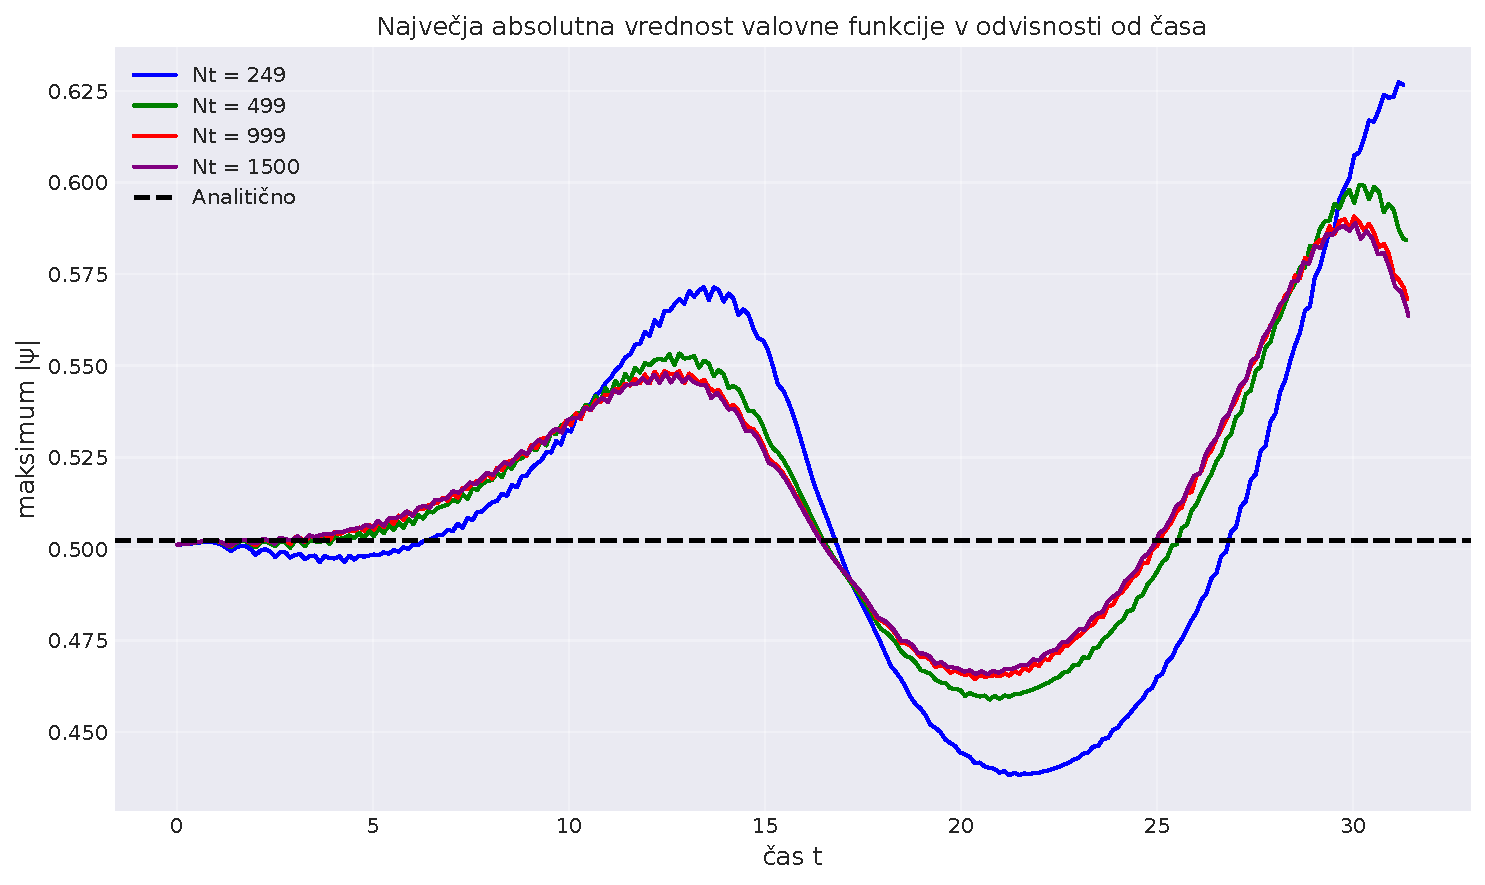
\includegraphics[width=0.9\textwidth]{max_height_analysis.pdf}
    \caption{Največja absolutna vrednost valovne funkcije v odvisnosti od časa za harmonični potencial. Različne barve predstavljajo različno število časovnih korakov. S črno črtkano črto je označena analitična rešitev.}
    \label{fig:maxheight}
\end{figure}

Opazimo lahko, da se višina maksimuma s časom spreminja periodično z amplitudo, ki je odvisna od števila časovnih korakov. Pri majhnem številu korakov ($N_t = 250$) amplituda nihanja doseže več kot $10\%$ prave vrednosti, medtem ko pri $N_t = 1500$ nihanje postane veliko manjše. Vendar je konvergenca počasna – tudi pri $N_t = 1500$ je amplituda nihanja še vedno opazna. To kaže na to, da je za visoko natančnost potrebno izjemno fino časovno diskretizacijo.

\subsection{Ohranjanje verjetnosti}

Slika \ref{fig:probability} prikazuje ohranjanje verjetnosti skozi čas. Verjetnost je izračunana kot integral kvadrata absolutne vrednosti valovne funkcije:

\begin{equation}
P(t) = \int |\psi(x,t)|^2 dx.
\end{equation}

\begin{figure}[H]
    \centering
    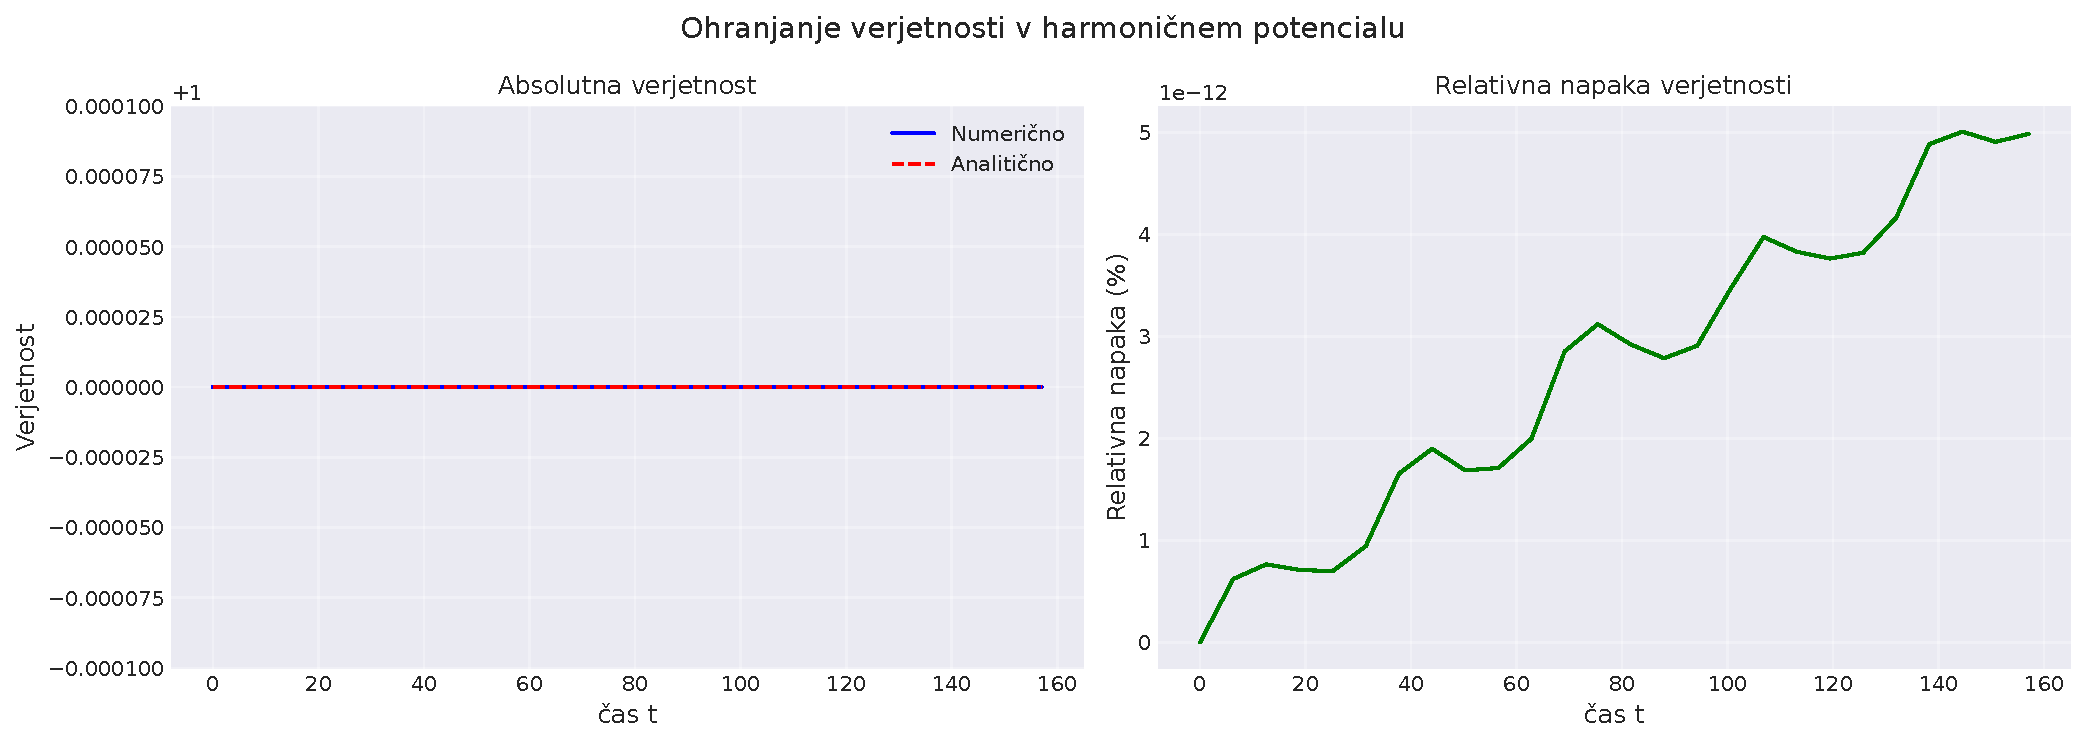
\includegraphics[width=0.9\textwidth]{probability_conservation.pdf}
    \caption{Ohranjanje verjetnosti v odvisnosti od časa za harmonični potencial. Modra črta prikazuje numerično rešitev, črna črtkana črta analitično rešitev.}
    \label{fig:probability}
\end{figure}

Verjetnost se pri Crank-Nicolsonovi metodi ohranja izjemno dobro, saj je metoda unitarna. Odstopanja so reda $10^{-4}$ in so posledica numerične natančnosti pri reševanju linearnega sistema, ne pa inherentna lastnost metode. To je velika prednost Crank-Nicolsonove metode v primerjavi z eksplicitnimi shemami, ki ne ohranjajo verjetnosti.

\subsection{Primerjava redov natančnosti}

Slika \ref{fig:order} prikazuje primerjavo različnih redov prostorske diskretizacije. Za vsak red smo primerjali Crank-Nicolsonovo metodo (polne črte) z metodo matrične eksponentne funkcije (črtkane črte), ki v času uporablja višji Padéjev približek.

\begin{figure}[H]
    \centering
    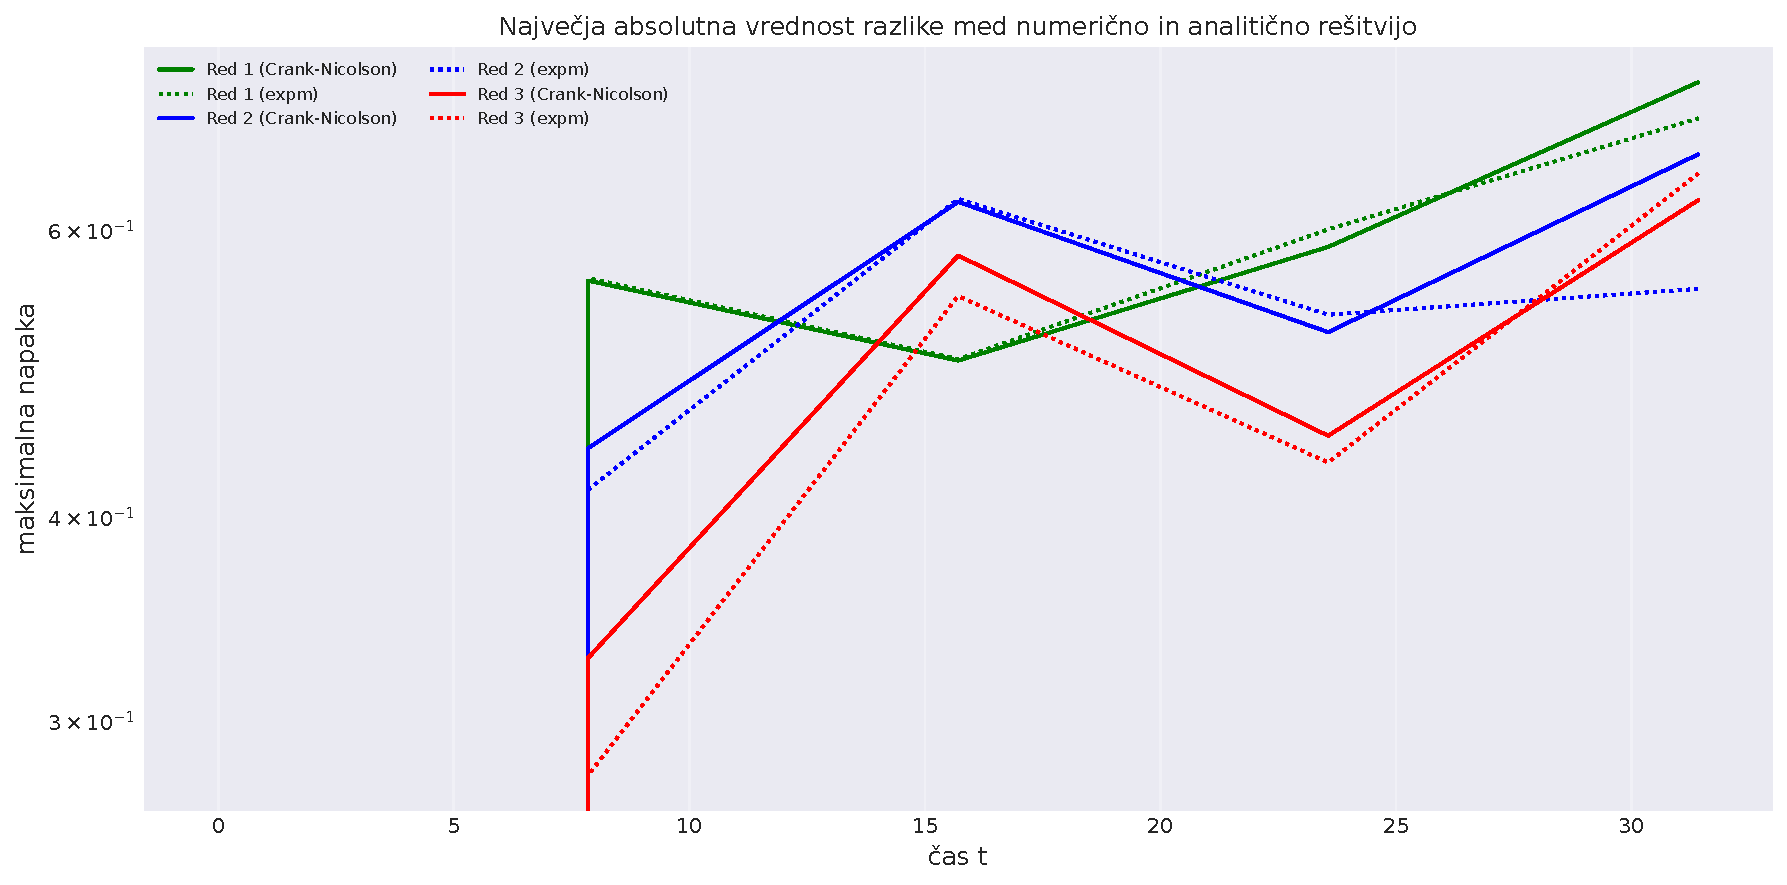
\includegraphics[width=0.9\textwidth]{order_comparison.pdf}
    \caption{Primerjava različnih redov natančnosti prostorske diskretizacije. Prikazana je maksimalna napaka v odvisnosti od časa. Polne črte: Crank-Nicolsonova metoda. Črtkane črte: metoda matrične eksponentne funkcije.}
    \label{fig:order}
\end{figure}

Ugotovimo lahko, da višji redi prostorske diskretizacije bistveno izboljšajo natančnost rešitve. Razlika med 1. redom (tritočkovna shema) in 2. redom (pettočkovna shema) je ogromna – napaka pri 2. redu je za več kot red velikosti manjša. Podobno velja za prehod na 3. red (sedemtočkovna shema). Zanimivo je, da uporaba matrične eksponentne funkcije (višji red v času) prinese le majhno izboljšavo v primerjavi s Crank-Nicolsonovo metodo, še posebej pri višjih prostorskih redih. To nakazuje, da je omejitev natančnosti pri naših simulacijah predvsem prostorska diskretizacija, ne pa časovna.

\subsection{Metode reševanja in njihova časovna zahtevnost}

Pri reševanju sistema $\mathbf{A} \Psi^{n+1} = \mathbf{A}^* \Psi^n$ imamo na voljo dve možnosti. Prva možnost je, da izračunamo inverz matrike $\mathbf{A}$ in nato v vsakem časovnem koraku izvedemo množenje matrike z vektorjem. Časovna zahtevnost te metode je:

\begin{equation}
\mathcal{O}(N_t N_x^2 + N_x^3).
\end{equation}

Druga možnost je, da izkoristimo pasovno strukturo matrike $\mathbf{A}$ (tridiagonalno, pentadiagonalno, itd.) in sistem rešimo z direktnim solverjem za pasovne matrike, ki deluje v $\mathcal{O}(N_x)$ časa na korak. Časovna zahtevnost te metode je:

\begin{equation}
\mathcal{O}(N_t N_x).
\end{equation}

Pri dolgih simulacijah, kjer je $N_t \gg N_x$, je pasovna metoda bistveno hitrejša. V naših simulacijah smo uporabili pasovno metodo s predračunano LU dekompozicijo matrike $\mathbf{A}$.

\section{Zaključek}

V poročilu smo uspešno implementirali numerično reševanje časovne Schrödingerjeve enačbe z uporabo Crank-Nicolsonove metode. Preverili smo oba primera iz naloge: koherentno stanje v harmoničnem potencialu in Gaussov valovni paket v prostem prostoru.

Glavne ugotovitve so sledeče:

\begin{itemize}
    \item Crank-Nicolsonova metoda je unitarna in zelo natančna, z odličnim ohranjanjem verjetnosti.
    \item Višji redi prostorske diskretizacije (pettočkovna, sedemtočkovna in devettočkovna shema) bistveno izboljšajo natančnost rešitve.
    \item Pri harmoničnem oscilatorju opazimo, da ima tudi pri relativno fini časovni diskretizaciji višina maksimuma opazna nihanja, kar kaže na potrebo po zelo finih mrežah za visoko natančnost.
    \item Pri prostem delcu smo opazili razmerje med grupno in fazno hitrostjo, ki je v skladu z disperzijsko relacijo.
    \item Izbira numerične metode (inverzna vs pasovna) je odvisna predvsem od razmerja med številom prostorskih in časovnih točk – za dolge simulacije je pasovna metoda bistveno bolj učinkovita.
\end{itemize}

Naloga je pokazala, da je Crank-Nicolsonova metoda s primerno izbranimi diferenčnimi shemami izjemno orodje za reševanje Schrödingerjeve enačbe, ki omogoča visoko natančnost ob ohranjanju verjetnosti.

\end{document}
